\documentclass[informe.tex]{subfiles}
\begin{document}


Un procedimiento para el diseño de filtros en otras estructuras diferentes a un filtro pasa bajo normalizado se consigue al trasladar los requerimientos de algunas estructuras de filtros no normalizadas a un filtro pasa bajo normalizado, para luego aplicar el procedimiento de diseño de un filtro pasa bajo normalizado, y finalmente, por medio de alguna función de transformación, se transforma la función de transferencia del filtro obtenido a la función de transferencia del filtro no normalizado de interés. Este procedimiento se resumen en la Fig.\ref{fig:transformacion:frecuencia:proceso}
				
		\begin{figure}[h]
		\centering
		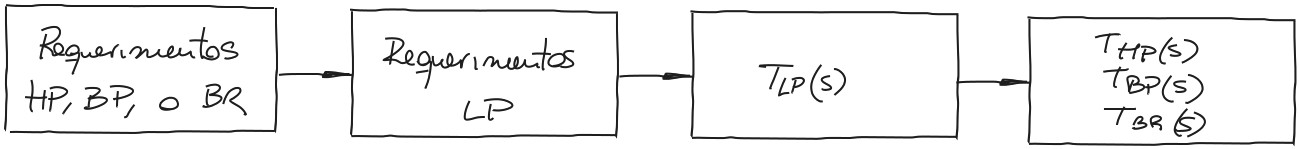
\includegraphics[scale=1.3]{transformacion_1.jpg}
		\caption{Procedimiento de diseño de un filtro no normalizado.}
		\label{fig:transformacion:frecuencia:proceso}
		\end{figure}

\end{document}	